\documentclass{beamer}
\usetheme{Madrid}
\usepackage{hyperref}
\usepackage{tikz}
\usetikzlibrary{arrows.meta,positioning,calendar}

\title{Trust Me, I am a Verifier!\\\vspace{0.3em}Interface Reliability Between Isabelle and External Provers}
\subtitle{Knowledge Exchange Projects - Amazon — Variant 3}
\author{Qilan Lin (K21204786)}
\institute{King's College London}
\date{2025--26}

\begin{document}

%------------------------------------------------
\begin{frame}
  \titlepage
\end{frame}

%------------------------------------------------
\begin{frame}{Agenda}
\begin{enumerate}
  \item Problem \& motivation
  \item Background: Sledgehammer pipeline
  \item Project goals \& research questions
  \item Proposed method: interface fuzzing
  \item Oracles, evaluation, risks, timeline
\end{enumerate}
\end{frame}

%------------------------------------------------
\begin{frame}{Problem Statement \& Motivation}
\begin{block}{Why this matters}
Sledgehammer is Isabelle/HOL’s main bridge to external ATP/SMT provers. It boosts proof automation but relies on a complex interface layer.
\end{block}

\begin{itemize}
  \item Interface bugs can cause crashes, hangs, or ``proof found'' results that fail to reconstruct.
  \item Translation/encoding choices (e.g., \texttt{lam\_trans}, \texttt{type\_enc}) trade power for robustness.
  \item Existing testing focuses on solvers; the Isabelle\(\leftrightarrow\)prover interface is under-tested.
\end{itemize}

\vspace{0.3em}
\textbf{Goal:} systematically stress-test this interface to improve reliability.
\end{frame}

%------------------------------------------------
\begin{frame}{Background: Sledgehammer at a Glance}
\begin{center}
\scalebox{0.64}{
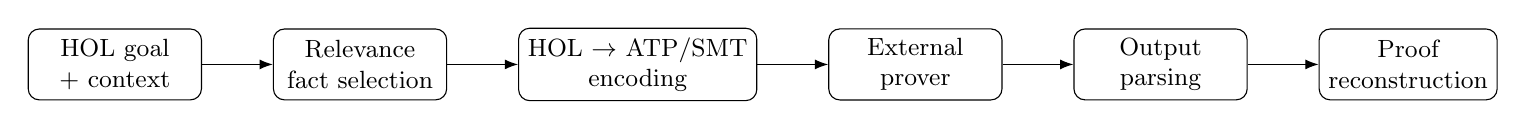
\begin{tikzpicture}[
  node distance=0.9cm,
  every node/.style={font=\small, align=center},
  box/.style={draw, rounded corners, minimum width=2.2cm, minimum height=0.9cm}
]

\node[box] (goal) {HOL goal\\+ context};
\node[box, right=of goal] (facts) {Relevance\\fact selection};
\node[box, right=of facts] (encode) {HOL \(\to\) ATP/SMT\\encoding};
\node[box, right=of encode] (prover) {External\\prover};
\node[box, right=of prover] (parse) {Output\\parsing};
\node[box, right=of parse] (recon) {Proof\\reconstruction};

\draw[-{Latex}] (goal) -- (facts);
\draw[-{Latex}] (facts) -- (encode);
\draw[-{Latex}] (encode) -- (prover);
\draw[-{Latex}] (prover) -- (parse);
\draw[-{Latex}] (parse) -- (recon);

\end{tikzpicture}
}
\end{center}

\begin{itemize}
  \item Variant 3 targets steps \textbf{3--5}: encoding, prover I/O, and reconstruction.
  \item These steps are where mismatches and robustness bugs typically arise.
\end{itemize}
\end{frame}

%------------------------------------------------
\begin{frame}{Where Interface Bugs Live}
\begin{columns}[T]
\column{0.48\textwidth}
\begin{block}{SUT-A: Encoding/Translation}
\begin{itemize}
  \item HOL \(\to\) TPTP / SMT-LIB
  \item Type and \(\lambda\)-abstraction encodings
  \item Risk: malformed or unsound-ish encodings
\end{itemize}
\end{block}

\column{0.48\textwidth}
\begin{block}{SUT-B/C: Prover I/O \& Reconstruction}
\begin{itemize}
  \item Process invocation, timeouts, parsing
  \item Metis/SMT proof replay
  \item Risk: ``proved'' but non-replayable, parser crashes
\end{itemize}
\end{block}
\end{columns}

\vspace{0.4em}
\textbf{Working assumption:} these layers contain latent edge-case bugs exploitable by systematically mutated inputs.
\end{frame}

%------------------------------------------------
\begin{frame}{Project Goals}
\begin{block}{High-level objective}
Build a fuzzer that targets Isabelle’s interface with external provers and quantitatively improves its bug-finding/testing coverage.
\end{block}

\textbf{Deliverables}
\begin{itemize}
  \item An interface-focused fuzzing framework and seed corpus.
  \item A set of minimized bug-revealing instances + reproduction scripts.
  \item Evaluation against baseline Sledgehammer usage.
\end{itemize}
\end{frame}

%------------------------------------------------
\begin{frame}{Research Questions}
\begin{itemize}
  \item \textbf{RQ1:} Can structure-aware mutation of Sledgehammer problems uncover crashes / hangs in the interface?
  \item \textbf{RQ2:} How often do mutated problems trigger prover inconsistencies (differential bugs)?
  \item \textbf{RQ3:} Which encodings/settings correlate with reconstruction failures?
  \item \textbf{RQ4:} Does the fuzzer outperform a baseline random/unaltered test suite in bug yield and interface-path diversity?
\end{itemize}
\end{frame}

%------------------------------------------------
\begin{frame}{Method Overview}
\begin{enumerate}
  \item \textbf{Seed extraction:} use Sledgehammer's CLI directly on AFP goals to export ATP/SMT problems (via \texttt{sledgehammer\_export}).
  \item \textbf{Structure-aware mutations:} generate syntactically valid variants (dictionary + grammar constraints).
  \item \textbf{Execution:} run multiple provers in parallel via the same Sledgehammer interface.
  \item \textbf{Oracles:} crash/hang, differential inconsistency, reconstruction failure.
  \item \textbf{Minimization:} delta-debugging to shrink bug instances.
\end{enumerate}
\end{frame}

%------------------------------------------------
\begin{frame}{Fuzzer Placement (Locked Down)}
\begin{block}{Main line (blackbox/greybox)}
\textbf{File-boundary fuzzing on exported TPTP / SMT-LIB problems.}
\end{block}

\begin{itemize}
  \item Inputs are exactly what the interface consumes (exported problems + prover outputs).
  \item Enables fast iteration without deep PolyML/Scala instrumentation.
  \item \textbf{MVP scope:} start with \textbf{SMT-LIB} exports + SMT provers (Z3, cvc5); 
        \textbf{extension:} add TPTP exports + ATPs (E, Vampire) once stable.
  \item Optional stretch: in-process fuzzing of the ML encoder.
\end{itemize}
\end{frame}

%------------------------------------------------
\begin{frame}{Seed Generation}
\begin{itemize}
  \item Select representative AFP sessions and goals.
  \item Use Sledgehammer's CLI directly with scripted batch export:
  \begin{itemize}
    \item multiple provers (E, Vampire, Z3, cvc5, \dots)
    \item encoding toggles: \texttt{lam\_trans}, \texttt{type\_enc}, time slices
    \item leverage \texttt{sledgehammer\_export\_smt} or custom ML script
  \end{itemize}
  \item \textbf{Phase 1 seeds:} prioritize SMT-LIB corpus to bootstrap AST-aware mutation.
  \item Store seeds + metadata (goal id, encoding, expected status).
\end{itemize}

\vspace{0.3em}
\textbf{Result:} a diverse real-world corpus of interface inputs.
\end{frame}

%------------------------------------------------
\begin{frame}{Mutation Strategy}
\begin{block}{Structure-aware mutational fuzzing}
Inspired by blackbox mutational SMT fuzzers (e.g., STORM) and type/grammar-aware mutation. 
\end{block}

\begin{itemize}
  \item \textbf{AST-first pipeline:} parse SMT-LIB/TPTP seeds to AST, mutate on-tree, then re-serialize 
        to keep \(\ge\)90\% mutants syntactically valid.
  \item Token-level edits: rename symbols, flip quantifiers, perturb numerals.
  \item Tree-level edits: swap subterms, duplicate/delete clauses.
  \item Constraint layer keeps formulas well-typed and valid:
  \begin{itemize}
    \item parentheses \& binder balance
    \item grammar/dictionary for each SMT theory / TPTP fragment
    \item type-aware operator substitution (avoid trivial ill-typed junk)
  \end{itemize}
\end{itemize}
\end{frame}

%------------------------------------------------
\begin{frame}{Related Work (Positioning)}
\begin{itemize}
  \item \textbf{Sledgehammer interface \& replay failures:} 
        Sledgehammer routinely reports ``proof found'' yet reconstruction can fail 
        (e.g., ``One-line proof reconstruction failed''), motivating interface-level testing.
  \item \textbf{Blackbox SMT fuzzing:} 
        STORM shows structure-aware mutation + minimization can expose real SAT/UNSAT soundness bugs.
  \item \textbf{Type/grammar-aware differential testing:}
        Type-aware AST mutation and cross-solver checking are highly effective for finding correctness bugs.
\end{itemize}
\end{frame}

%------------------------------------------------
\begin{frame}{Bug Oracles}
\begin{itemize}
  \item \textbf{Crash/Hang Oracle}
  \begin{itemize}
    \item Isabelle/Sledgehammer exception, prover crash, or hard timeout.
  \end{itemize}
  \item \textbf{Differential Oracle}
  \begin{itemize}
    \item Same input, different provers/settings return inconsistent results.
    \item \textbf{Noise filters (standard in SMT differential testing):}
      \begin{itemize}
        \item count only \textbf{SAT vs UNSAT / proved vs disproved} as correctness conflicts;
        \item treat \texttt{unknown}/timeout as performance signals, not bugs;
        \item re-run conflicts to confirm reproducibility.
      \end{itemize}
  \end{itemize}
  \item \textbf{Reconstruction Oracle}
  \begin{itemize}
    \item External prover succeeds but Isabelle replay fails (officially known Sledgehammer failure class).
    \item Track failure rate \textbf{by encoding knobs} and Metis/SMT replay strategy.
  \end{itemize}
\end{itemize}

\vspace{0.3em}
Each oracle yields a saved test case for minimization.
\end{frame}

%------------------------------------------------
\begin{frame}{Minimization \& Reporting}
\begin{itemize}
  \item Use delta-debugging to shrink failing instances.
  \item Normalize to a smallest reproducible core (for developer triage).
  \item Generate a bug report bundle:
  \begin{itemize}
    \item seed id + mutation trace
    \item prover logs and Isabelle reconstruction trace
    \item one-command reproducer
  \end{itemize}
\end{itemize}
\end{frame}

%------------------------------------------------
\begin{frame}{Implementation Plan}
\begin{itemize}
  \item \textbf{Driver:} Python-based fuzzer runner.
  \item \textbf{Isabelle hooks:} export problems, invoke provers consistently.
  \item \textbf{Prover pool:} local installs + Isabelle wrappers.
  \item \textbf{Storage:} corpus, coverage proxies, failure database.
\end{itemize}

\vspace{0.3em}
\textbf{Prototype milestone:} end-to-end loop working on a small AFP subset.
\end{frame}

%------------------------------------------------
\begin{frame}{MVP Demo Plan (30--60 seconds)}
\begin{enumerate}
  \item \textbf{Export a real SMT-LIB seed} from a small AFP goal via Sledgehammer CLI
  \begin{itemize}
    \item show 1 script/command + resulting \texttt{.smt2} file (metadata: goal, encoding knobs).
  \end{itemize}

  \item \textbf{Run the fuzzer for a tiny budget} (e.g., 100--500 mutants, Z3 vs cvc5)
  \begin{itemize}
    \item screen shows: mutants generated $\rightarrow$ provers invoked $\rightarrow$ logs collected.
  \end{itemize}

  \item \textbf{Show 1 concrete find} and how the oracle fires
  \begin{itemize}
    \item either \textbf{(a)} SAT/UNSAT conflict confirmed by re-run, or
    \item \textbf{(b)} ``proved'' but \textbf{replay fails} (official Sledgehammer failure class).
    \item {\scriptsize Differential rule-of-thumb: only count \textbf{SAT vs UNSAT} as correctness bugs; 
          \texttt{unknown}/timeout are filtered as performance signals.}
  \end{itemize}

  \item \textbf{Minimization output}
  \begin{itemize}
    \item show before/after size + one-command reproducer in the bug bundle.
  \end{itemize}
\end{enumerate}
\end{frame}

%------------------------------------------------
\begin{frame}{Evaluation}
\begin{block}{Baseline}
Run Sledgehammer on the same goals without mutation (standard batch testing).
\end{block}

\textbf{Metrics}
\begin{itemize}
  \item Unique crashes/hangs found.
  \item Unique differential correctness conflicts found.
  \item Reconstruction failure rate by encoding / replay strategy.
  \item \textbf{Interface-path coverage proxy:}
    \begin{itemize}
      \item number of unique exception sites / outcome categories triggered across
            encoding, prover I/O, parsing, replay;
      \item compare baseline vs fuzzer to show new interface paths exercised.
    \end{itemize}
  \item Time-to-first-bug, bugs/hour, corpus diversity.
\end{itemize}
\end{frame}

%------------------------------------------------
\begin{frame}{Risks \& Mitigations}
\begin{itemize}
  \item \textbf{Too many invalid mutants} $\rightarrow$ AST/grammar constraints + repair.
  \item \textbf{Search space explosion} $\rightarrow$ prioritization by novelty and failure history.
  \item \textbf{Tooling/installation friction} $\rightarrow$ pin Isabelle release + Docker fallback.
  \item \textbf{Hard-to-triage failures} $\rightarrow$ aggressive minimization and full logs.
\end{itemize}
\end{frame}

%------------------------------------------------
\begin{frame}{Expected Contributions}
\begin{itemize}
  \item First systematic fuzzer focused on the Isabelle\textendash prover interface.
  \item A reusable seed corpus of Sledgehammer-exported problems.
  \item Bug reports / patches improving stability and trustworthiness.
  \item Empirical map of \textbf{which encoding knobs correlate with replay failures}.
\end{itemize}
\end{frame}

%------------------------------------------------
\begin{frame}{Timeline (Indicative)}
\begin{center}
\scalebox{0.75}{
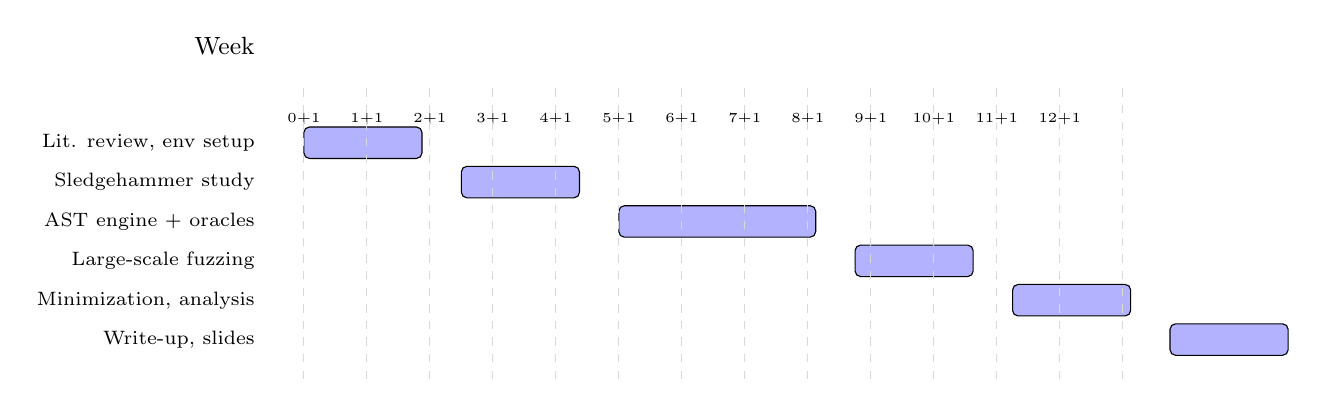
\begin{tikzpicture}[
    gantt/.style={draw, fill=blue!30, minimum height=0.6cm, rounded corners=2pt},
    ganttlabel/.style={anchor=east, font=\scriptsize},
    weeklabel/.style={font=\tiny, anchor=north}
]
    % Week labels
    \foreach \x in {0,...,12} {
        \node[weeklabel] at (\x*0.8, 4) {\x+1};
    }
    \node[anchor=south east, font=\small] at (-0.5, 4.5) {Week};
    
    % Task bars
    \node[ganttlabel] at (-0.5, 3.5) {\scriptsize Lit. review, env setup};
    \draw[gantt] (0, 3.3) rectangle (1.5, 3.7);
    
    \node[ganttlabel] at (-0.5, 3.0) {\scriptsize Sledgehammer study};
    \draw[gantt] (2, 2.8) rectangle (3.5, 3.2);
    
    \node[ganttlabel] at (-0.5, 2.5) {\scriptsize AST engine + oracles};
    \draw[gantt] (4, 2.3) rectangle (6.5, 2.7);
    
    \node[ganttlabel] at (-0.5, 2.0) {\scriptsize Large-scale fuzzing};
    \draw[gantt] (7, 1.8) rectangle (8.5, 2.2);
    
    \node[ganttlabel] at (-0.5, 1.5) {\scriptsize Minimization, analysis};
    \draw[gantt] (9, 1.3) rectangle (10.5, 1.7);
    
    \node[ganttlabel] at (-0.5, 1.0) {\scriptsize Write-up, slides};
    \draw[gantt] (11, 0.8) rectangle (12.5, 1.2);
    
    % Grid lines
    \foreach \x in {0,...,13} {
        \draw[gray!30, dashed] (\x*0.8, 0.5) -- (\x*0.8, 4.2);
    }
\end{tikzpicture}
}
\end{center}
\end{frame}

%------------------------------------------------
\begin{frame}{Timeline (Detailed)}
\begin{tabular}{ll}
Weeks 1--2 & Literature review, environment setup \\
Weeks 3--4 & Sledgehammer pipeline study, seed export script \\
Weeks 5--7 & AST mutation engine + oracles, end-to-end prototype \\
Weeks 8--9 & Large-scale fuzzing campaigns \\
Weeks 10--11 & Minimization, bug triage, analysis \\
Weeks 12--13 & Write-up, slides, final evaluation \\
\end{tabular}
\end{frame}

%------------------------------------------------
\begin{frame}{Summary}
\begin{itemize}
  \item Variant 3 targets a high-impact but under-tested layer.
  \item Main method: file-boundary, AST/grammar-aware mutational fuzzing.
  \item Strong oracles + systematic evaluation make results publishable.
\end{itemize}

\vspace{0.5em}
\textbf{Immediate Next Steps}
\begin{itemize}
  \item Implement Sledgehammer CLI scripting for batch seed extraction
  \item Implement core mutation operators (AST-aware)
  \item Set up prover pool and test harness
  \item Begin Phase 1 evaluation on SMT-LIB corpus
\end{itemize}
\end{frame}

\end{document}
